\section{Proofs}
\label{app:proofs}

Throughout, $m\equiv\alpha_T(1-\alpha_D)$ and all derivatives are evaluated at a balanced free-trade baseline (\cref{app:linear}).

\begin{proof}[Proof of \cref{lem:gs}]
Trade balances are measured in the common unit of account of \cref{sec:bilateral}. Scaling every currency value $v_l$, $l\in\mathcal I$, by a common factor leaves all relative prices unchanged and scales every common-unit income, and hence every flow $f_{ij}$ and trade balance $\TB_i$, by the same factor, so $\TB_i$ is homogeneous of degree one in currency values. By Euler's theorem $\sum_{l\in\mathcal I}\widetilde J_{il}=\TB_i$, which is zero at the balanced baseline. Summing \cref{eq:tb} over $i\in\mathcal I$ gives $\sum_{i\in\mathcal I}\TB_i\equiv0$, so $\sum_{i\in\mathcal I}\widetilde J_{il}=0$. By gross substitutability, $\widetilde J_{il}\geq0$ for $l\neq i$, so $\widetilde J_{ii}=-\sum_{l\neq i}\widetilde J_{il}\leq0$. Since $\nu_l=\chi_l-\chi_A$ and $\chi_A$ is fixed by $v_A=1$, the reduced matrix is $J=(\widetilde J_{il})_{i,l\in\mathcal I_{-A}}$, obtained by deleting row and column $A$. Its off-diagonal entries are nonnegative, and for each $i\in\mathcal I_{-A}$
\begin{equation*}
|J_{ii}|-\sum_{l\in\mathcal I_{-A},\,l\neq i}J_{il}=\widetilde J_{iA}\geq0,
\end{equation*}
with strict inequality in every row $i\in\mathcal I_{-A}$ for which $\widetilde J_{iA}>0$, and by hypothesis there is at least one such row. Row $A$ plays no role, because it is deleted from the reduced system. Thus $-J$ is a Z-matrix that is weakly diagonally dominant, irreducible, and strictly diagonally dominant in at least one row. Its diagonal is strictly positive, since $|J_{ii}|=0$ would force row $i$ of $J$ to vanish, contradicting irreducibility. Write $-J=D-K$ with $D=\operatorname{diag}(-J)>0$ and $K\geq0$. Every row sum of $D^{-1}K$ is at most one and at least one is strictly below one; with irreducibility, its spectral radius is $r<1$. Hence $(-J)^{-1}=(I-D^{-1}K)^{-1}D^{-1}=\sum_{k\geq0}(D^{-1}K)^kD^{-1}\geq0$ componentwise, nonsingularity follows from $r<1$, and $\det(-J)=\det D\cdot\det(I-D^{-1}K)>0$.
\end{proof}

\begin{proof}[Proof of \cref{prop:decomposition}]
Let $M$ be an $(N-1)\times(N-1)$ matrix with $PMP'=M$ for every permutation matrix $P$. Conjugating by the transposition of $i$ and $j$ gives $M_{ii}=M_{jj}$, and conjugating by a permutation that sends the ordered pair $(i,j)$ to $(k,l)$, $i\neq j$, $k\neq l$, gives $M_{ij}=M_{kl}$. Hence $M=aI+b\bone\bone'$. Since $\bone'\bone=N-1$ and $\bone'v=0$ for zero-sum $v$, $(aI+b\bone\bone')\bone=(a+(N-1)b)\bone$ and $(aI+b\bone\bone')v=av$. For $-J=a_JI+b_J\bone\bone'$ and $G^{(A)}=a_GI+b_G\bone\bone'$ this gives $j_S=a_J+(N-1)b_J$, $j_D=a_J$, $g_S=a_G+(N-1)b_G$ and $g_D=a_G$. For $j_S,j_D\neq0$,
\begin{equation*}
(-J)^{-1}=\frac{1}{j_D}I+\frac{1}{N-1}\Big(\frac{1}{j_S}-\frac{1}{j_D}\Big)\bone\bone',
\end{equation*}
as direct multiplication verifies. Thus $(-J)^{-1}$ and $G^{(A)}$ share the one-dimensional common eigenspace $\operatorname{span}\{\bone\}$ and the $(N-2)$-dimensional zero-sum eigenspace, with response coefficients $\lambda_{\mathrm{avg}}=g_S/j_S$ and $\lambda_{\mathrm{rel}}=g_D/j_D$; applying them to $t=\bar t\bone+\widetilde t$ gives \cref{eq:decomp}. Because $\widetilde t$ sums to zero, it does not affect the equally weighted average of the responses, which under partner symmetry is $d\nu^E_A$ (\cref{sec:decomposition}); this gives the first equality in \cref{eq:decompparts}; the second is immediate, and for any two partners $d\log e_{jk}=d\nu_k-d\nu_j=\lambda_{\mathrm{rel}}(\widetilde t_k-\widetilde t_j)=\lambda_{\mathrm{rel}}(t_k-t_j)$.

For the MML characterization, which uses the permutation symmetry throughout, MML requires (a) the Z-matrix sign pattern, $J_{il}\geq0$ for $l\neq i$, and (b) a nonsingular $-J$ with $(-J)^{-1}\geq0$ componentwise. (a) The off-diagonal entry of $-J$ is $b_J=(j_S-j_D)/(N-1)$, so (a) holds if and only if $j_D\geq j_S$. (b) Given $j_D\geq j_S>0$, $-J$ is nonsingular, the diagonal entries $1/j_D+(1/j_S-1/j_D)/(N-1)$ and the off-diagonal entries $(1/j_S-1/j_D)/(N-1)$ of $(-J)^{-1}$ above are nonnegative, so MML holds. Conversely, if MML holds, (a) gives $j_D\geq j_S$, and since $-J$ is nonsingular and $(-J)^{-1}\bone=\bone/j_S$ must be nonnegative, $j_S>0$.
\end{proof}

\begin{proof}[Proof of \cref{thm:main}]
At the symmetric benchmark the primitives and the balanced baseline are invariant to every relabeling of $A$'s partners, so $PJP'=J$ and $PG^{(A)}P'=G^{(A)}$ for every partner permutation $P$, and \cref{prop:decomposition} applies. By \cref{lem:jacobian}, $j_S=mM_N/(N-1)$ and $j_D=Nj_S$, so $j_S>0$ if and only if $M_N>0$, in which case $j_D>j_S$; by \cref{prop:decomposition}, MML is therefore equivalent to $M_N>0$. If $\eta\geq1$, every term in the bracket of \cref{eq:MN} is nonnegative and the first is one, so $M_N>0$. Given $M_N>0$, dividing \cref{eq:geigen} by the eigenvalues in \cref{eq:Jsym} gives $\lambda_{\mathrm{avg}}=-\rho_D/M_N$ and $\lambda_{\mathrm{rel}}=-\rho/(NM_N)$, and \cref{eq:lambdas} is \cref{eq:decomp}.
\end{proof}

\begin{proof}[Proof of \cref{prop:unilateral}]
The three responses are derived in \cref{app:linear}. Under MML $M_N>0$, and $\rho_D>0$, so $d\nu^E_A<0$ and $d\nu_B<0$, and, for every individual bystander $c$, $d\nu_c>0$ if and only if $\rho>N\rho_D$. Part (iv) is \cref{eq:kpartners,eq:reltreat}.
\end{proof}

\begin{proof}[Proof of \cref{cor:single}]
Let $\alpha_D\geq1/N$. Both terms on the right of \cref{eq:single} are nonnegative, so $N\rho_D\geq\eta$, and $\rho>N\rho_D$ implies $\rho>\eta$. With $\rho=\eta=\sigma$, \cref{eq:unilateral} gives $d\nu_c/d\tau=(\sigma-N\rho_D)/[N(N-1)M_N]$, and by \cref{eq:single}, $\sigma-N\rho_D=-[\sigma(N\alpha_D-1)+N(1-\alpha_D)(1-\alpha_T)]\leq0$. Under MML $M_N>0$, so $d\nu_c/d\tau\leq0$. The bracket is a sum of two nonnegative terms, and since $\sigma>0$ and $\alpha_D<1$ it vanishes if and only if $\alpha_D=1/N$ and $\alpha_T=1$. At $\alpha_D=1/N$, $M_N=\sigma$ and $d\nu_c/d\tau=-(1-\alpha_T)/(N\sigma)$ (\cref{app:linear}), which is identically zero when $\alpha_T=1$.
\end{proof}

\paragraph{The complete three-region mapping.} \Cref{prop:composite} applies to any tariff change that is invariant to permutations of the $N-2$ bystanders, that is, any combination of tariffs by $A$ or $B$ that are common across all bystanders, tariffs by all bystanders on $A$ or on $B$ that are common across bystanders, and tariffs between $A$ and $B$. Such a shock maps into the three-region economy by $d\tau_{AC}=d\tau_{Ac}$, $d\tau_{CA}=d\tau_{cA}$, $d\tau_{BC}=d\tau_{Bc}$ and $d\tau_{CB}=d\tau_{cB}$, the common values across bystanders, with $d\tau_{AB}$ and $d\tau_{BA}$ retained. The three-region economy $\{A,B,C\}$ is a nested-CES economy in which:
\begin{itemize}
\item $C$ has income $y_C=N-2$;
\item $A$ and $B$ place import weight $\frac{1}{N-1}$ on each other and $\frac{N-2}{N-1}$ on $C$;
\item $C$ places weight $\tfrac12$ on each of $A$ and $B$ within its import nest, and retains the tradable expenditure share $\alpha_T$ and the cross-origin elasticity $\rho$;
\item $C$'s home share of tradables is $h_C=\alpha_D+(1-\alpha_D)\frac{N-3}{N-1}$, equivalently $(N-1)h_C=N-3+2\alpha_D$;
\item $C$'s home--import elasticity is $\eta_C$ in \cref{eq:etaC}.
\end{itemize}
Given $M_N\neq0$, equivalently $j_S=mM_N/(N-1)\neq0$, the linearized systems of the two economies have the same solution for $d\nu_B$, the common bystander response $d\nu_c=d\nu_C$, and $A$'s NEER. The equivalence is first-order: it concerns the linearized systems and need not hold along nonlinear paths at finite tariffs. For $N=3$, $C$ is the single bystander, with $y_C=1$, $h_C=\alpha_D$ and $\eta_C=\eta$.

\begin{proof}[Proof of \cref{prop:composite}]
Let $N\geq3$ and label the countries $A$, $B$ and bystanders $c=1,\dots,N-2$. Consider any tariff change in the class described in the proposition, and write the composite economy's variables with a capital $C$. The argument compares the two linearized systems at the symmetric benchmark; it establishes that they are identical, not that the nonlinear economies coincide at finite tariffs.

\emph{Step 1: bystanders move together.} The baseline and the shock are invariant to permutations of the bystanders. By \cref{lem:jacobian}, $-J=j_S(NI-\bone\bone')$ has eigenvalues $j_S$ and $Nj_S$, so for $j_S\neq0$ the linearized system \cref{eq:JG} is nonsingular and has a unique solution. That solution is therefore invariant to the same permutations, so $d\nu_c=d\nu_C$ for every bystander. The equilibrium is then characterized by two conditions, $d\TB_B=0$ and $\sum_cd\TB_c=0$ (each $d\TB_c$ is equal across bystanders), in the two unknowns $(d\nu_B,d\nu_C)$.

\emph{Step 2: the baseline flows coincide.} In the $N$-country economy $f_{Ac}=f_{cA}=m/(N-1)$ for each bystander, so $\sum_cf_{Ac}=\sum_cf_{cA}=m(N-2)/(N-1)$. In the composite, $f_{AC}=\alpha_T(1-\alpha_D)\frac{N-2}{N-1}=m\frac{N-2}{N-1}$, and, since $1-h_C=2(1-\alpha_D)/(N-1)$, $f_{CA}=\alpha_T(1-h_C)\cdot\frac12\cdot(N-2)=m\frac{N-2}{N-1}$. The same holds for $B$, and $f_{AB}=f_{BA}=m/(N-1)$ in both economies. In particular the composite is balanced, and $s_{CA}=\alpha_T(1-h_C)/2=m/(N-1)=s_{cA}$.

\emph{Step 3: $A$'s and $B$'s demand aggregate exactly.} All bystander goods face the same price change in $A$, $dp_{Ac}=d\nu_C+d\tau_{Ac}$ with $d\tau_{Ac}$ common across $c$. Hence $d\log P_{MA}=\frac{1}{N-1}dp_{AB}+\frac{N-2}{N-1}dp_{Ac}$, which is the composite's index with $b_{AC}=\frac{N-2}{N-1}$, and $d\log s_{Ac}=(1-\rho)(dp_{Ac}-d\log P_{MA})+(1-\eta)\alpha_D\,d\log P_{MA}$ is common across $c$ and equal to the composite's $d\log s_{AC}$. $A$'s income response, $d\log\tilde I_A=s_{AB}d\tau_{AB}+\sum_cs_{Ac}d\tau_{Ac}$, equals the composite's because $\sum_cs_{Ac}=s_{AC}$. Therefore $\sum_cdf_{Ac}=df_{AC}$, and likewise $df_{AB}$ is the same in both economies; the same argument applies to $B$.

\emph{Step 4: intra-bloc trade cancels.} Summing \cref{eq:tb} over bystanders,
\begin{equation*}
\sum_c\TB_c=\sum_c(f_{Ac}+f_{Bc})-\sum_c(f_{cA}+f_{cB})+\Big[\sum_c\sum_{c'\neq c}f_{c'c}-\sum_c\sum_{c'\neq c}f_{cc'}\Big],
\end{equation*}
and the bracket is identically zero. So $\sum_c\TB_c$ has the form of the composite's $\TB_C=f_{AC}+f_{BC}-f_{CA}-f_{CB}$, and $\TB_B=f_{AB}+\sum_cf_{cB}-f_{BA}-\sum_cf_{Bc}$ has the form of the composite's $\TB_B$. Given Step 3, it remains to show $\sum_cdf_{cA}=df_{CA}$ and $\sum_cdf_{cB}=df_{CB}$.

\emph{Step 5: the bloc's demand for $A$'s and $B$'s goods.} Since $d\log f_{cA}=d\log s_{cA}+d\log\tilde I_c-d\tau_{cA}$ and all three terms are common across bystanders, $\sum_cdf_{cA}=(N-2)f_{cA}\,d\log f_{cA}=f_{CA}\,d\log f_{cA}$; we need $d\log f_{cA}=d\log f_{CA}$. Incomes: $d\log\tilde I_c=d\nu_C+s_{cA}d\tau_{cA}+s_{cB}d\tau_{cB}$, which equals $d\log\tilde I_C$ because $s_{CA}=s_{cA}$ and $s_{CB}=s_{cB}$ (Step 2). Tariff wedges: $d\tau_{cA}=d\tau_{CA}$ by construction. Shares: measure prices in bystander currency, so that other bystanders' goods have $dp=0$, and write $dp_{cA}=\frac{S+D}{2}$ and $dp_{cB}=\frac{S-D}{2}$, where $S\equiv dp_{cA}+dp_{cB}$ and $D\equiv dp_{cA}-dp_{cB}$. A bystander's import price index moves by $S/(N-1)$, since $A$ and $B$ are two of its $N-1$ equally weighted origins. Hence
\begin{equation*}
\begin{aligned}
d\log s_{cA}&=(1-\rho)\Big(\frac{S+D}{2}-\frac{S}{N-1}\Big)+(1-\eta)\alpha_D\frac{S}{N-1}\\
&=(1-\rho)\frac D2+\Big[(1-\rho)\frac{N-3}{2(N-1)}+(1-\eta)\frac{\alpha_D}{N-1}\Big]S.
\end{aligned}
\end{equation*}
In the composite the import index moves by $S/2$, so $d\log s_{CA}=(1-\rho)\frac D2+(1-\eta_C)h_C\frac S2$. The $D$ terms coincide for any $(S,D)$, and the $S$ terms coincide if and only if $(1-\eta_C)(N-1)h_C=(1-\rho)(N-3)+2\alpha_D(1-\eta)$. Using $(N-1)h_C=N-3+2\alpha_D$, this is \cref{eq:etaC}. The argument for $B$'s good is identical with $D$ replaced by $-D$. The residual share on bloc goods matches as well, because shares sum to one in both economies.

\emph{Step 6: equilibrium and NEER.} By Steps 2--5, the two equations $(d\TB_B,\sum_cd\TB_c)=0$ of the $N$-country economy, evaluated at $d\nu_c=d\nu_C$, are identical to the composite's equations $(d\TB_B,d\TB_C)=0$, including the tariff terms. For $j_S\neq0$ the composite system is nonsingular (its determinant is computed in Step 7), so the two linearized systems have the same solution $(d\nu_B,d\nu_C)$. The composite's trade weights are $w_{AB}=1/(N-1)$ and $w_{AC}=(N-2)/(N-1)$, so its NEER response $\frac{1}{N-1}d\nu_B+\frac{N-2}{N-1}d\nu_C$ equals the $N$-country NEER at symmetric weights.

\emph{Step 7: the reduced system.} By \cref{lem:jacobian}, row $B$ of $-J$ in the $N$-country economy is $j_S(N-1)$ on $\nu_B$ and $-j_S$ on each bystander's rate; imposing $d\nu_c=d\nu_C$ gives $(j_S(N-1),-j_S(N-2))$. Each bystander row has $-j_S$ on $\nu_B$, $j_S(N-1)$ on its own rate and $-j_S$ on each of the other $N-3$ bystanders' rates; summing the $N-2$ bystander rows and imposing $d\nu_c=d\nu_C$ gives $(-j_S(N-2),\,(N-2)[j_S(N-1)-j_S(N-3)])=(-j_S(N-2),2j_S(N-2))$. The reduced system for $(\nu_B,\nu_C)$ is therefore
\begin{equation}
-J=j_S\begin{pmatrix}N-1&-(N-2)\\-(N-2)&2(N-2)\end{pmatrix},\qquad \det(-J)=j_S^2N(N-2),
\label{eq:reducedJ}
\end{equation}
since $j_S^2[2(N-1)(N-2)-(N-2)^2]=j_S^2N(N-2)$; for $N\geq3$ the determinant is positive if and only if $j_S\neq0$. Let $F_B$ be the target's disturbance, $F_c$ that of an individual bystander, and $F_C=\sum_cF_c=(N-2)F_c$ the aggregate disturbance of the composite. For $j_S\neq0$, inverting \cref{eq:reducedJ} and applying it to $(F_B,F_C)$ gives
\begin{equation}
d\nu_C=\frac{F_B+(N-1)F_c}{Nj_S},\qquad d\nu_B=\frac{2F_B+(N-2)F_c}{Nj_S},
\label{eq:reducedsol}
\end{equation}
where $d\nu_C$ is the common response $d\nu_c$ of every bystander; the unilateral disturbances follow from \cref{eq:disturbance}. For $N=3$ there is one bystander, $(N-1)h_C=2\alpha_D$ gives $h_C=\alpha_D$, and \cref{eq:etaC} gives $\eta_C=\eta$, so the composite is that bystander.
\end{proof}

Under a unilateral tariff, $F_B=-m[\rho_D+(N-2)\rho]/(N-1)^2<0$, while $F_c$ is given by \cref{eq:FC} and is positive only when $\rho>\rho_D$. In \cref{eq:reducedsol}, the bystanders' positive disturbance pushes toward a depreciation of $A$ against them, while the target's negative disturbance works in the opposite direction, because the target's depreciation makes its goods cheaper to the bystanders. Under MML, $A$ depreciates against the bystanders if and only if
\begin{equation*}
(N-1)(\rho-\rho_D)>\rho_D+(N-2)\rho\quad\Longleftrightarrow\quad\rho>N\rho_D.
\end{equation*}

\paragraph{An ordinary-$\eta$ composite.} As a diagnostic comparison, which is not part of \cref{prop:composite}, consider an ordinary-$\eta$ composite. It holds $y_C$, $h_C$, $A$'s and $B$'s import weights, the baseline external bilateral flows and the trade weights at their mapped $N$-country values, replaces $\eta_C$ by $\eta$, and leaves $\rho$ unchanged. Its bystander threshold falls slightly with $N$, in line with the local, calibration-dependent finding of \cref{app:asym-primitives} that a marginally larger bystander lowers the threshold near the symmetric point, whereas the true threshold $N\rho_D$ rises steeply (\cref{tab:composite,fig:composite}). The $N$-dependence therefore comes from the bloc's internal trade, governed by $\rho$, rather than from the bloc's size.

\noindent The replication code verifies the reduction numerically: for $(\alpha_D,\alpha_T,\eta)$ equal to $(0.8,0.4,1.5)$, $(0.6,0.7,1.2)$, $(0.9,0.3,3.0)$ and $(0.5,0.5,2.0)$, $N\in\{4,\dots,10\}$ and $\rho\in\{1.1,4,9\}$, under the four shocks ($A$ on $B$; an $A$--$B$ war; $A$ on all bystanders; all bystanders on $B$), the composite's $(d\nu_B,d\nu_C)$ match the $N$-country responses to within $10^{-12}$. \Cref{tab:composite} reports the bystander thresholds plotted in \cref{fig:composite}.

\begin{table}[ht]
\centering
\caption{$N$ versus bystander size}
\label{tab:composite}
\begin{tabular}{ccccc}
\toprule
 & & \multicolumn{2}{c}{Composite bystander threshold} & \\
\cmidrule(lr){3-4}
$N$ & $N\rho_D$ (true) & with $\eta_C$ \cref{eq:etaC} & with ordinary $\eta$ & $\eta_C$ at $\rho=4$ \\
\midrule
\tabinput{tables/tab1_composite.tex}
\bottomrule
\end{tabular}

\vspace{4pt}
\begin{minipage}{0.92\textwidth}\footnotesize
\textit{Notes:} Illustrative US-like calibration ($\alpha_D=0.8$, $\alpha_T=0.4$, $\eta=1.5$). Thresholds are the values of $\rho$ at which the bystander response to a unilateral tariff changes sign in the composite economy of \cref{prop:composite}, computed with the linear system of \cref{app:linear}. The ordinary-$\eta$ column keeps the composite's mapped flows, weights and $\rho$ but replaces $\eta_C$ by $\eta$, as in the ordinary-$\eta$ composite above.
\end{minipage}
\end{table}

\begin{figure}[ht]
\centering
\begin{subfigure}[t]{0.47\textwidth}\centering
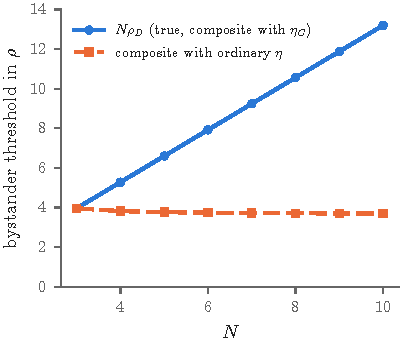
\includegraphics[width=\textwidth]{fig4a_composite_threshold.pdf}
\caption{Bystander threshold}
\end{subfigure}\hfill
\begin{subfigure}[t]{0.47\textwidth}\centering
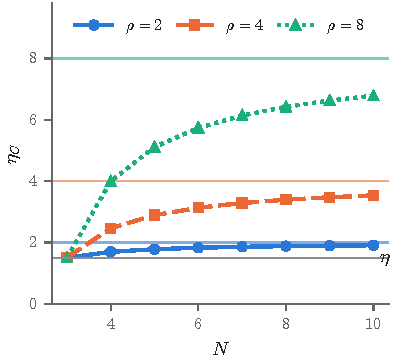
\includegraphics[width=\textwidth]{fig4b_eta_C.pdf}
\caption{Effective elasticity $\eta_C$}
\end{subfigure}
\caption{The composite bystander. (a) The bystander threshold $N\rho_D$, which the composite with $\eta_C$ reproduces, and the threshold of the ordinary-$\eta$ composite, for $N=3,\dots,10$. (b) $\eta_C$ for $\rho\in\{2,4,8\}$, converging toward $\rho$ (thin horizontal lines); the grey line is $\eta=1.5$. \textit{Notes:} illustrative US-like calibration $\alpha_D=0.8$, $\alpha_T=0.4$, $\eta=1.5$.}
\label{fig:composite}
\end{figure}

\begin{proof}[Proof of \cref{prop:real}]
\Cref{eq:realapp,eq:reer} are derived in \cref{app:linear}. For a unilateral tariff $\bar t=d\tau/(N-1)$, so $d\log q_{Ac}/d\tau=(1-\frac{mN}{N-1})\,d\nu_c/d\tau-\frac{m}{N-1}$. Substituting $d\nu_c/d\tau$ from \cref{eq:unilateral} and writing $\frac{m}{N-1}=\frac{mN\,M_N}{N(N-1)M_N}$ gives
\begin{equation*}
\frac{d\log q_{Ac}}{d\tau}=\frac{H_N(\rho)}{N(N-1)M_N(\rho)}.
\end{equation*}
Where MML holds, $M_N>0$, so the response has the sign of $H_N$. Since $\rho_D$ does not depend on $\rho$ and $M_N(\rho)$ in \cref{eq:MN} has slope $dM_N/d\rho=(N-2)/(N-1)$, $H_N$ is affine in $\rho$ with slope
\begin{equation*}
\frac{dH_N}{d\rho}=1-\frac{mN}{N-1}-\frac{mN(N-2)}{N-1}=1-mN.
\end{equation*}

(i) If $m<1/N$, the slope is positive, so $H_N$ has a unique root, is negative below it and positive above it. Multiplying $H_N=0$ by $N-1$ gives $[(N-1)-mN](\rho-N\rho_D)=mN[1+N\alpha_D(\eta-1)+(N-2)\rho]$; the coefficient on $\rho$ is $(N-1)-mN-mN(N-2)=(N-1)(1-mN)$, which yields $\rho^*_q(N)$. At the root $[(N-1)-mN](\rho^*_q-N\rho_D)=mN(N-1)M_N(\rho^*_q)$. For $m<1/N$ the coefficient $(N-1)-mN$ is positive, and if MML holds at $\rho^*_q$ the right-hand side is positive, so $\rho^*_q(N)>N\rho_D$.

(ii) If $m=1/N$, the slope is zero, and
\begin{equation*}
H_N=\frac{N-2}{N-1}(\rho-N\rho_D)-\frac{1+N\alpha_D(\eta-1)+(N-2)\rho}{N-1}=-\frac{1+N\alpha_D(\eta-1)+N(N-2)\rho_D}{N-1}.
\end{equation*}

(iii) If $m>1/N$, the slope is negative.

(iv) If $\eta\geq1$, every term of $M_N$ in \cref{eq:MN} is nonnegative and the first is positive, so MML holds for every $\rho>0$. Since $(N-1)M_N(0)=1+N\alpha_D(\eta-1)$,
\begin{equation*}
(N-1)H_N(0)=-[(N-1)-mN]N\rho_D-mN[1+N\alpha_D(\eta-1)]=-N\big[(N-1)(\rho_D-m)+Nm^2\big],
\end{equation*}
where the second equality uses $\rho_D=1+\alpha_D(\eta-1)-m$. With $\eta\geq1$, $\rho_D-m=1+\alpha_D(\eta-1)-2m\geq1-2m$, so
\begin{align*}
(N-1)(\rho_D-m)+Nm^2&\geq(N-1)(1-2m)+Nm^2=Nm^2-2(N-1)m+(N-1)\\
&=N\Big(m-\frac{N-1}{N}\Big)^2+\frac{N-1}{N}>0.
\end{align*}
Hence $H_N(0)<0$. For $m\geq1/N$, $dH_N/d\rho=1-mN\leq0$, so $H_N(\rho)\leq H_N(0)<0$ and $d\log q_{Ac}/d\tau<0$ for every $\rho>0$.

(v) Under MML $M_N>0$, and $\rho_D>0$. In \cref{eq:reer}, the first term is nonpositive when $m\leq(N-1)/N$ and the second, $-m/(N-1)$, is strictly negative, so the REER strictly appreciates, including at $m=(N-1)/N$. Under weak home bias, $m=\alpha_T(1-\alpha_D)\leq1-1/N=(N-1)/N$.
\end{proof}

\begin{proof}[Proof of \cref{prop:retaliation}]
(i) Let primes denote responses to the mirror shock $t_{BA}=d\tau$. Relabeling $A\leftrightarrow B$ in \cref{eq:unilateral} gives
\begin{equation*}
d\log e'_{BA}=-\frac{N\rho_D+(N-2)\rho}{N(N-1)M_N}\,d\tau,\qquad d\log e'_{Bc}=\frac{\rho-N\rho_D}{N(N-1)M_N}\,d\tau.
\end{equation*}
Since $e_{AB}=1/e_{BA}$ and $e_{Ac}=e_{AB}e_{Bc}$, $d\log e'_{AB}=\frac{N\rho_D+(N-2)\rho}{N(N-1)M_N}d\tau$ and $d\log e'_{Ac}=\frac{\rho}{NM_N}d\tau$. By linearity the combined response is $d\log e_{AB}=0$ and
\begin{equation*}
d\log e_{Ac}=\frac{\rho-N\rho_D}{N(N-1)M_N}\,d\tau+\frac{\rho}{NM_N}\,d\tau=\frac{\rho-\rho_D}{(N-1)M_N}\,d\tau.
\end{equation*}
The three components are $A$'s average protection, $-\rho_D/[(N-1)M_N]$, $A$'s relative treatment, $\rho/[N(N-1)M_N]$, and $B$'s relative treatment, $\rho/(NM_N)$. By symmetry between $A$ and $B$ the same expression applies to $d\log e_{Bc}$, every bystander moves identically, so cross rates among bystanders are unchanged, and averaging over $A$'s $N-1$ partners with the equal weights of the symmetric benchmark gives $d\nu^E_A$ in \cref{eq:retaliation}.

(ii) Superpose the $N$ tariff vectors. $A$'s tariff vector is uniform, $\bar t^{(A)}=d\tau$ and $\widetilde t^{(A)}=0$, and contributes $\lambda_{\mathrm{avg}}d\tau$ to every $d\log e_{Aj}$. Partner $j$ taxes only $A$; its contribution to $d\log e_{Aj}$ is $-[\lambda_{\mathrm{avg}}+(N-2)\lambda_{\mathrm{rel}}]\frac{d\tau}{N-1}$, while each of the $N-2$ other partners $k$ contributes $-\lambda_{\mathrm{rel}}d\tau=\frac{\rho}{NM_N}d\tau$, computed as in part (i) from $e_{Aj}=e_{Ak}e_{kj}$. Summing,
\begin{equation*}
d\log e_{Aj}=\lambda_{\mathrm{avg}}d\tau-\big[\lambda_{\mathrm{avg}}+(N-2)\lambda_{\mathrm{rel}}\big]\frac{d\tau}{N-1}-(N-2)\lambda_{\mathrm{rel}}d\tau=\frac{(N-2)(\rho-\rho_D)}{(N-1)M_N}\,d\tau.
\end{equation*}
The expression is the same for every $j$, so it equals the effective response, and all cross rates among $A$'s partners are unchanged. Under MML the signs are those of $\rho-\rho_D$.
\end{proof}

\begin{proof}[Proof of \cref{lem:welfare}]
Utility is Cobb--Douglas over the tradable aggregate and the non-tradable, so indirect utility is $V_A=\kappa\,I_A/(P_{TA}^{\alpha_T}P_{NA}^{1-\alpha_T})$ for a constant $\kappa$, with $I_A$, $P_{TA}$ and $P_{NA}$ in $A$'s currency. The marginal utility of income is $V_A/I_A$, so the change in welfare in units of income is
\begin{equation*}
\frac{dV_A}{(\partial V_A/\partial I_A)\,I_A}=d\log I_A-\alpha_T\,d\log P_{TA}-(1-\alpha_T)\,d\log P_{NA}.
\end{equation*}
This is the envelope theorem: by Shephard's lemma, $\alpha_T\,d\log P_{TA}=\sum_j s_{Aj}\,d\log p_{Aj}$, the expenditure-share-weighted change in consumer prices. Under the producer-price normalization $w_A=A_{TA}$ and $P_{NA}=A_{TA}/A_{NA}$ are fixed in $A$'s currency, so $d\log P_{NA}=0$ and the domestic tradable's price does not move. Imported goods' consumer prices move by $d\log p_{Aj}=d\nu_j+d\log(1+\tau_{Aj})=d\nu_j+d\tau_{Aj}$ at free trade. Income is labor income plus rebated revenue, $I_A=w_AL_A/(1-\sum_j\theta_{Aj}s_{Aj})$ with $\theta_{Aj}=\tau_{Aj}/(1+\tau_{Aj})$. At free trade $\theta_{Aj}=0$ and $d\theta_{Aj}=d\tau_{Aj}$, so changes in realized shares drop out and $d\log I_A=\sum_js_{Aj}\,d\tau_{Aj}$: the revenue gain equals the tariff change times the border value of imports. Combining,
\begin{equation*}
\frac{dV_A}{(\partial V_A/\partial I_A)\,I_A}=\sum_js_{Aj}\,d\tau_{Aj}-\sum_js_{Aj}(d\nu_j+d\tau_{Aj})=-\sum_js_{Aj}\,d\nu_j=-m_A\sum_{j\neq A}b_{Aj}\,d\nu_j,
\end{equation*}
with $m_A=\sum_js_{Aj}=\alpha_T(1-h_A)$ and $b_{Aj}=s_{Aj}/m_A$. The tariff terms cancel: at free trade the revenue raised exactly offsets the direct price increase to first order. Tariffs imposed by other countries enter $A$'s prices and income only through $d\nu$, so the formula holds for any tariff vector.
\end{proof}

\noindent The replication code checks \cref{lem:welfare} against central finite differences of $A$'s log indirect utility in the nonlinear model, at symmetric and asymmetric free-trade baselines ($N=3,4,5$) and under unilateral, retaliatory, multilateral-war, foreign-only and random tariff shocks; the two agree to within $10^{-6}$.

\begin{proof}[Proof of \cref{prop:uniform}]
Work with the linearized system \cref{eq:linear} at a balanced free-trade baseline, with country-specific $\eta_i$, $\rho_i$ and $\alpha_T^i$, so that $s_{Aj}=\alpha_T^A(1-h_A)b_{Aj}$ and $m_A=\sum_{j\neq A}s_{Aj}=\alpha_T^A(1-h_A)$.

\emph{Step 1: only $A$'s import flows are disturbed.} Set $d\nu=0$ and $d\tau_{Aj}=dt$ for all $j\neq A$, with all other tariff changes zero. For $i\neq A$, $d\tau_{ij}=0$, so $dp_{ij}=0$ for every $j$, $d\log P_{Mi}=0$, $d\log s_{ij}=0$ and $d\log\tilde I_i=0$. Every flow $f_{ij}$ with $i\neq A$ is therefore unchanged. In the trade balance of partner $j$, the only term that moves is its exports to $A$:
\begin{equation*}
F_j=d\TB_j\big|_{d\nu=0}=f_{Aj}\big(d\log s_{Aj}+d\log\tilde I_A-dt\big).
\end{equation*}

\emph{Step 2: the cross-origin margin drops out.} In $A$, $dp_{Aj}=dt$ for every $j$, so $d\log P_{MA}=\sum_jb_{Aj}dt=dt$ and $dp_{Aj}-d\log P_{MA}=0$ for every $j$. The term multiplying $(1-\rho_A)$ vanishes, and
\begin{equation*}
d\log s_{Aj}=(1-\eta_A)h_A\,dt\quad\text{for every }j,\qquad d\log\tilde I_A=\sum_js_{Aj}\,dt=m_A\,dt.
\end{equation*}

\emph{Step 3: the disturbance.} Substituting,
\begin{equation*}
F_j=f_{Aj}\big[(1-\eta_A)h_A+\alpha_T^A(1-h_A)-1\big]dt=-f_{Aj}\big[\eta_Ah_A+(1-h_A)(1-\alpha_T^A)\big]dt=-f_{Aj}\,\rho_D^A\,dt,
\end{equation*}
which is \cref{eq:uniformF}. Since $\eta_A>0$, $0<h_A\leq1$ and $\alpha_T^A\leq1$, $\rho_D^A>0$, so $F_j\leq0$ for every $j$, with $F_j<0$ whenever $f_{Aj}>0$.

\emph{Step 4: exchange rates.} Under MML, $(-J)^{-1}\geq0$, so by \cref{eq:signrule} $d\nu_i=\sum_j\vartheta_{ij}F_j\leq0$ for every $i$: $A$ appreciates weakly against every partner. If $A$ imports from every partner, then $F_j<0$ for all $j$; since $(-J)^{-1}$ is nonsingular and nonnegative, each of its rows has a strictly positive entry, so $d\nu_i<0$ for every $i$. If instead $J$ is irreducible, $-J$ is an irreducible nonsingular M-matrix and $(-J)^{-1}>0$ entrywise, so $d\nu_i<0$ for every $i$ as long as $F\neq0$, that is, as long as $A$ imports at all.

\emph{Step 5: welfare.} By \cref{lem:welfare}, $dU_A/(U_A'I_A)=-m_A\sum_jb_{Aj}d\nu_j\geq0$, and it is strictly positive whenever some $d\nu_j<0$ with $b_{Aj}>0$, which holds in either case of Step 4 because the $b_{Aj}$ sum to one. Since $A$'s aggregate terms of trade improve if and only if $\sum_jb_{Aj}d\nu_j<0$, they improve. Finally, the response is linear in the tariff vector, so the welfare effect of the uniform tariff is $\sum_jg_j\,dt$ with $g_j$ as in \cref{eq:gradient}, and $\sum_jg_j>0$.
\end{proof}

\noindent The replication code checks \cref{eq:uniformF} against the linear system to $10^{-12}$ and against complex-step derivatives of the exact model's trade balances, and verifies the signs of $F$, $d\nu$ and the welfare change on 60 random asymmetric baselines with country-specific parameters ($N=3,4,5$).

\begin{proof}[Proof of \cref{prop:threecases}]
Under MML $\det A(\rho)>0$, so $R_{A|B}$ has the sign of $Q_{A|B}(\rho)$. (a) At the symmetric benchmark, \cref{eq:threecountry} gives $\det A=3(mM_3/2)^2$ and $R_{A|B}=d\nu^E_A/d\tau=-\rho_D/(2M_3)$, so $Q=-\tfrac38m^2\rho_DM_3$, which is affine in $\rho$ ($q_2=0$) and negative for all $\rho$ under MML. (b) If $q_2>0$ and $q_0<0$, the product of the roots is $q_0/q_2<0$, so there is exactly one positive root $\rho^*$, with $Q<0$ on $(0,\rho^*)$ and $Q>0$ beyond. (c) If $q_2<0$, $q_1>0$, $q_0<0$ and the discriminant is positive, both roots are real with positive sum $-q_1/q_2$ and positive product $q_0/q_2$, so both are positive, and the downward parabola is positive only between them.
\end{proof}
